%%%%%%%%%%%%%%%%%%%%%%%%%
% Dokumentinformationen %
%%%%%%%%%%%%%%%%%%%%%%%%%
\newcommand{\titleinfo}{Wahrscheinlichkeitsrechnung und Statistik - Formelsammlung}
\newcommand{\authorinfo}{Braun \& Co, J.Rast, H.Badertscher}
\newcommand{\versioninfo}{$Revision: 2 $ - powered by \LaTeX}  

%%%%%%%%%%%%%%%%%%%%%%%%%%%%%%%%%%%%%%%%%%%%%
% Standard projektübergreifender Header für
% - Makros 
% - Farben
% - Mathematische Operatoren
%
% DORT NUR ERGÄNZEN, NICHTS LÖSCHEN\newpage
%%%%%%%%%%%%%%%%%%%%%%%%%%%%%%%%%%%%%%%%%%%%%
% Genereller Header
\documentclass[10pt,twoside,a4paper,fleqn]{article}
% Dateiencoding
\usepackage[utf8]{inputenc}
% Seitenränder
\usepackage[left=1cm,right=1cm,top=1cm,bottom=1cm,includeheadfoot]{geometry}
% Sprachpaket
\usepackage[ngerman]{babel,varioref}

% Pakete
\usepackage{amssymb,amsmath,fancybox,graphicx,color,lastpage,wrapfig,fancyhdr,hyperref,verbatim,floatflt,multicol,multirow,rotating,pdflscape,array,longtable,listings}

% Zum Bilder einfach in Tabellen einfügen (valign=t)
\usepackage[export]{adjustbox}

%%%%%%%%%%%%%%%%%%%%
% Generelle Makros %
%%%%%%%%%%%%%%%%%%%%
\newcommand{\skript}[1]{$_{\textcolor{red}{\mbox{\small{Skript S.#1}}}}$}
\newcommand{\verweis}[2]{\small{(siehe auch \ref{#1}, #2 (S. \pageref{#1}))}}
\newcommand{\verweiskurz}[1]{(\small{siehe \ref{#1}\normalsize)}}
\newcommand{\subsubadd}[1]{\textcolor{black}{\mbox{#1}}}
\newcommand{\formelbuch}[1]{$_{\textcolor{red}{\mbox{\small{S#1}}}}$}

\newcommand{\kuchling}[1]{$_{\textcolor{red}{\mbox{\small{Kuchling #1}}}}$}
\newcommand{\stoecker}[1]{$_{\textcolor{grey}{\mbox{\small{Stöcker #1}}}}$}
\newcommand{\sachs}[1]{$_{\textcolor{blue}{\mbox{\small{Sachs S. #1}}}}$}
\newcommand{\hartl}[1]{$_{\textcolor{green}{\mbox{\small{Hartl S. #1}}}}$}


\newcommand{\skriptsection}[2]{\section{#1 {\tiny Skript S. #2}}}
\newcommand{\skriptsubsection}[2]{\subsection{#1 {\tiny Skript S. #2}}}
\newcommand{\skriptsubsubsection}[2]{\subsubsection{#1 {\tiny Skript S. #2}}}

\newcommand{\matlab}[1]{\footnotesize{(Matlab: \texttt{#1})}\normalsize{}}

%%%%%%%%%%
% Farben %
%%%%%%%%%%
\definecolor{black}{rgb}{0,0,0}
\definecolor{red}{rgb}{1,0,0}
\definecolor{white}{rgb}{1,1,1}
\definecolor{grey}{rgb}{0.8,0.8,0.8}
\definecolor{green}{rgb}{0,.8,0.05}
\definecolor{brown}{rgb}{0.603,0,0}

%%%%%%%%%%%%%%%%%%%%%%%%%%%%
% Mathematische Operatoren %
%%%%%%%%%%%%%%%%%%%%%%%%%%%%
\DeclareMathOperator{\sinc}{sinc}
\DeclareMathOperator{\sgn}{sgn}
\DeclareMathOperator{\Real}{Re}
\DeclareMathOperator{\Imag}{Im}
\DeclareMathOperator{\e}{e}
\DeclareMathOperator{\cov}{cov}
\DeclareMathOperator{\PolyGrad}{PolyGrad}


%%%%%%%%%%%%%%%%%%%%%%%%%%%
% Fouriertransformationen %
%%%%%%%%%%%%%%%%%%%%%%%%%%%
\unitlength1cm
% Zeitbereich -- Frequenzbereich
\newcommand{\laplace}
{
\begin{picture}(1,0.5)
\put(0.2,0.1){\circle{0.14}}\put(0.27,0.1){\line(1,0){0.5}}\put(0.77,0.1){\circle*{0.14}}
\end{picture}
}
% Frequenzbereich -- Zeitbereich
\newcommand{\Laplace}
{
\begin{picture}(1,0.5)
\put(0.2,0.1){\circle*{0.14}}\put(0.27,0.1){\line(1,0){0.45}}\put(0.77,0.1){\circle{0.14}}
\end{picture}
}

% Fouriertransformationen
\unitlength1cm
\newcommand{\FT}
{
\begin{picture}(1,0.5)
\put(0.2,0.1){\circle{0.14}}\put(0.27,0.1){\line(1,0){0.5}}\put(0.77,0.1){\circle*{0.14}}
\end{picture}
}


\newcommand{\IFT}
{
\begin{picture}(1,0.5)
\put(0.2,0.1){\circle*{0.14}}\put(0.27,0.1){\line(1,0){0.45}}\put(0.77,0.1){\circle{0.14}}
\end{picture}
}




%%%%%%%%%%%%%%%%%%%%%%%%%%%%
% Allgemeine Einstellungen %
%%%%%%%%%%%%%%%%%%%%%%%%%%%%
%PDF Info
\hypersetup{pdfauthor={\authorinfo},pdftitle={\titleinfo},colorlinks=false}
\author{\authorinfo}
\title{\titleinfo}

%%%%%%%%%%%%%%%%%%%%%%%
% Kopf- und Fusszeile %
%%%%%%%%%%%%%%%%%%%%%%%
\pagestyle{fancy}
\fancyhf{}
%Linien oben und unten
\renewcommand{\headrulewidth}{0.5pt} 
\renewcommand{\footrulewidth}{0.5pt}

\fancyhead[L]{\titleinfo{ }\tiny{(\versioninfo)}}
%Kopfzeile rechts bzw. aussen
\fancyhead[R]{Seite \thepage { }von \pageref{LastPage}}
%Fusszeile links bzw. innen
\fancyfoot[L]{\footnotesize{\authorShort}}
%Fusszeile rechts bzw. ausen
\fancyfoot[R]{\footnotesize{\today}}
% Lizenz CC-BY-NC-SA
% Headerfile für die Einbindung einer Lizenzgrafik in den Footer
% Verwendung: \lizenz{cc-by-nc-sa}{small}
\newcommand{\lizenz}[2]
{
\fancyfoot[C]{
  \includegraphics[width=1.6cm]{./header/lizenzen/#1/#2.png} \quad $\rightarrow$ \href{https://github.com/HSR-Stud}{Github: HSR-Stud}
}
}
\lizenz{cc-by-nc-sa}{small}
% Einrücken verhindern versuchen
\setlength{\parindent}{0pt}

% Zeilenhöhe Tabellen:
\newcommand{\arraystretchOriginal}{1.5}
\renewcommand{\arraystretch}{\arraystretchOriginal}


\usepackage[usenames,dvipsnames]{xcolor}
\usepackage{tikz}
\usetikzlibrary{arrows,decorations.pathmorphing,positioning,fit,petri}
\usetikzlibrary{calc,intersections,through,backgrounds,graphs}
\usetikzlibrary{patterns,decorations.pathreplacing}


% Möglichst keine Ergänzungen hier, sondern in header.tex
\begin{document}
%%%%%%%%%%%%%%%%%%%%%%%%%%%%%%%%%%%%%%%%%%%%%%%%%%%%%%%%%%%%%%%%%%%%%%%%%%%%%%%%%%%%%%%%%%%%%%%%
%%%%%%%%%%%%%%%%%%%%%%%%%%%%%%%%%%%%%%%%%%%%%%%%%%%%%%%%%%%%%%%%%%%%%%%%%%%%%%%%%%%%%%%%%%%%%%%%
\section{Ereignisse und ihre Wahrscheinlichkeit}

\subsection{Kombinatorik \skript{5} \sachs{66}}
\begin{tabular}{| p{5.5cm} | c | c |}
  \hline
  Art der Auswahl bzw. Zusammenstellung von $k$ aus $n$ Elementen &
  \multicolumn{2}{|c|}{Anzahl der Möglichkeiten} \\
  & ohne Wiederholungen & mit Wiederholungen \\
 	&	$(k\leq n)$         & $(k\leq n)$ \\
 	\hline
 	Permutationen & $P_n=n!\quad(n=k)$       & $P_n^{(k)}=\frac{n!}{k!}$ \\
 	Kombinationen & $C_n^{(k)}=\binom n k$   & $C_n^{(k)}=\binom{n+k-1} k$ \\
  Variationen   & $V_n^{(k)}=k!\binom n k$ & $V_n^{(k)}=n^k$\\
  \hline
\end{tabular}
\begin{list}{$\bullet$}{\setlength{\itemsep}{0cm} \setlength{\parsep}{0cm}
\setlength{\topsep}{0.1cm}}
  \item \textbf{Permutationen}: Gegeben seien $n$ verschiedene Objekte. Dann
    gibt es $n!$ verschiedene Reihenfolgen in denen man diese Objekte anordnen
    kann. \\
    z.B.: $x,y,z;\quad x,z,y;\quad z,y,x;\ldots$
  \item \textbf{Kombination}: Gegeben seien $n$ verschiedene Objekte. Dann gibt
    es $\binom n k$ Möglichkeiten, daraus $k$ Objekte auszuwählen, wenn es nicht
    auf die Reihenfolge ankommt. \\
    z.B.: Wie viele verschiedene Möglichkeiten hat man beim Lotto, 6 Zahlen aus
    49 auszuwählen?
  \item \textbf{Variation} nennt man eine Auswahl von $k$ Elementen aus $n$
    verschiedenen Elementen unter Beachtung der Reihenfolge
\end{list}
\hrule

\subsection{Wahrscheinlichkeit \& Rechenregeln \skript{32}}
\begin{tabular}{ll}
  Wertebereich:         & ${0}\le{P(A)}\le{1}$\\
  Sicheres Ereignis:    & $P(\Omega)=1$\\
  unmögliches Ereignis: & $P(\emptyset)=0$
\end{tabular}
		\begin{tabular}{ll}
			komplementär Ereignis:
			&$P(\bar{A})=P({\Omega}\setminus{A})=1-P(A)$\\
			Differenz der Ereignisse A und B:
			&$P({A}\setminus{B})=P(A)-P({A}\cap{B})$\\
			Vereinigung zweier Ereignisse:
			&$P({A}\cup{B})=P(A)+P(B)-P({A}\cap{B})$
		\end{tabular}
\hrule

\subsection{Unabhängige Ereignise \skript{36} \sachs{83}}
		Unabhängige Ereignisse $A$ und $B$ liegen vor, wenn: \hspace*{5mm} $P(A\mid
		B)=P(A)$ \hspace{4mm} und \hspace{4mm} $P(B\mid A)=P(B)$ \hspace*{5mm} erfüllt
		ist. \\
		Für sie gilt \hspace*{5mm} $P(A\cap B)=P(A)P(B)$\\
    	Die Tatsache, dass A eingetreten ist, hat keinen Einfluss auf die 
		Wahrscheinlichkeit von B.\\
\hrule

\subsection{Bedingte Wahrscheinlichkeit \skript{35} \sachs{85}}
Die Wahrscheinlichkeit für das Eintreten des Ereignisses $A$ unter der
Bedingung, dass das Ereignis $B$ bereits eingetreten ist.
\begin{center}
  $P(A\mid B)= \dfrac{P(A\cap B)}{P(B)}=\underbrace{\frac{P(A)\cdot
  P(B)}{P(B)}=P(A)}_{\text{nur wenn unabhängig}}$
\end{center}
\hrule

\subsection{Satz von Bayes \skript{43} \sachs{89}}
\begin{tabular}{ll}
  $P(B\mid A)=P(A\mid B) \cdot\dfrac{P(B)}{P(A)}$
  \vspace{1mm}
\end{tabular}
\hrule

\subsection{Laplace-Ereignisse \skript{47} \sachs{79}}
In einem endlichen Wahrscheinlichkeitsraum $\Omega$ haben alle
Elementarereignisse die gleiche Wahrscheinlichkeit.
\begin{center}
  $P(A)=\dfrac{\left| A\right|}{\left|\Omega\right|}$
\end{center}
\hrule

\subsection{Totale Wahrscheinlichkeit \skript{58 ???} \sachs{88}}
\begin{tabular}{ll}
  $P(A)=\sum\limits_{i=1}^N P(A\mid G_i)\cdot P(G_i)$
\end{tabular}

\section{Erwartungswert und Varianz}

\subsection{Erwartungswert \skript{63} \sachs{101}}
Sei $X$ eine Funktion auf $\Omega$, und lasse sich $\Omega$ in endlich viele
Ereignisse, auf denen $X(\omega)$ konstant ist, $A_i$ zerlegen, dann ist der
Erwartungswert von $X$ \\
\hspace*{5.7cm}
$Erwartungswert = \sum Wert \cdot Wahrscheinlichkeit$ \\
\hspace*{7.5cm}
$E(X)=\sum\limits_{i=0}^n \underbrace{X(A_i)}_{\text{Wert}}\cdot
\underbrace{P(A_i)}_{\text{W'keit}}$ \\
\hspace*{5.7cm}
$E(X) = \int\limits_{-\infty}^x x \cdot \varphi(x) dx$ mit $\varphi(x) =
Dichtefunktion$

\subsubsection{Rechenregeln \skript{67}}
\begin{tabular}{ll}
  $E(X+Y)=E(X)+E(Y)$ \\
  $E(\lambda X + \mu) = \lambda \cdot E(X) + \mu$ & $\lambda, \mu \in
  \mathbb{R}$ \\
  $E(XY) = E(X)\cdot E(Y)$ & wenn X,Y unabhängig sind \\
\end{tabular}
\vspace{1mm} %
\hrule       % <<- Wär tuet so scheiss??
\vspace{2mm} %

\begin{minipage}{9cm}
\subsection{Varianz \skript{63} \sachs{106}}
  \begin{tabular}{ll}
    $var(x)=\sigma ^2=E[(X-E(X))^2]=E(X^2)-E(X)^2$\\
	\end{tabular}
	\subsubsection{Kovarianz \sachs{49}}
	\begin{tabular}{ll}
	  $cov(X,Y)=E(XY)-E(X)E(Y)=\underbrace{0}_{\text{falls X,Y unabhängig}}$
	\end{tabular}
\end{minipage}
\begin{minipage}{9cm}
  \subsubsection{Rechenregeln}
  \begin{tabular}{ll}
    $var(\lambda X)=\lambda^2 var(X) \qquad $ $\lambda, \mu
    \in \mathbb{R}$\\
    $var(X_1+X_2+\ldots+X_n) \neq var(n X)$ \\
    $var(X+Y)= \begin{cases}
      var(X)+var(Y)                      &	\text{(X,Y unabh.)}\\                     
      var(X) + var(Y) + 2 \cdot cov(X,Y) &	\text{(X,Y abhängig)}\\
    \end{cases} $ \\
    $var(X Y)= var(Y)var(X)+var(Y)E(X)^2+var(X)E(Y)^2$
  \end{tabular}
\end{minipage}
\vspace{1mm}
\hrule

\subsection{Erwartungswert und Varianz des arithmetischen Mittels \skript{78}}
Es sei eine folge von unabhängigen Zufallsvariablen $X_1, X_2, \ldots , X_n$ mit
gleichem Erwartungswert $ \mu $ und gleicher Varianz $ \sigma^2 $ gegeben. \\
\begin{tabular}{p{6cm} p{6cm} p{6cm}}
  Mittelwert: $M_n=\frac{X_1+\ldots+X_n}{n}$ &
  Erwartungswert: $E(X)=E(M_n)$ &
  Varianz: $var(M_n)=\frac{1}{n}var(X)$
\end{tabular}
\vspace{1mm}
\hrule
\vspace{2mm}

\begin{minipage}[]{9cm}
  \subsection{Regression \skript{80} \sachs{60, 141}}
  \begin{tabular}{ll}
    Allgemein: & X,Y Zufallsvariable \\
    Gesucht: & Regressionsgerade $y=ax+b$ mit min. Fehler \\
    Fehler: & $E(Y-(aX+b))=0$
  \end{tabular}
  \vspace{.1cm}
  \textbf{Regressionskoeffizient r} \\
  $r$ ist ein Mass für die Qualität der Regression (standardisiert) \\
  $r^2=\dfrac{cov(X,Y)^2}{var(X)var(Y)}$ \\
  \textbf{Mittlerer quadratischer Fehler} \\
  $\Delta^2 = var(Y)(1-r^2) =
  var(Y)\left(1-\dfrac{cov(X,Y)^2}{var(X)var(Y)}\right) $ \\
\end{minipage}
\begin{minipage}{10cm}
  \textbf{Vorgehen:}
  \textcolor{grey}{mit Fehlerberechnung}
	\begin{enumerate}
		\item Tabelle mit bekannten Werten aufstellen:\\
  		\begin{tabular}{|l||l|l||l|l||l|}
  		  \hline
        \textbf{$k$} & \textbf{$x$} & \textbf{$x^2$} & \textbf{$y$} &
  		  \textcolor{grey}{\textbf{$y^2$}} & \textbf{$xy$} \\
  		  \hline \hline
  		  $1$ & $x_1$ & $x_1^2$ & $y_1$ & \textcolor{grey}{$y_1^2$} & $x_1y_1$ \\
  		  \hline
  		  $\vdots$ & $\vdots$ & $\vdots$ & $\vdots$ & \textcolor{grey}{$\vdots$} &
  		  $\vdots$ \\\hline $n$ & $x_n$ & $y_n^2$ & $y_n$ & \textcolor{grey}{$y_n^2$} & $x_ny_n$ \\
  		  \hline
  		  \hline
  		  $\sum$ & $\sum x_k$ & $\sum x_k^2$ & $\sum y_k$ & \textcolor{grey}{$\sum
  		  y_k^2$} & $\sum x_ky_k$ \\
  		  \hline $E$ & $\frac{\sum x_k}{n}$ & $\frac{\sum x_k^2}{n}$ & $\frac{\sum
  		  y_k}{n}$ & \textcolor{grey}{$\frac{\sum y_k^2}{n}$} & $\frac{\sum x_ky_k}{n}$ \\
  		  \hline
  		\end{tabular} 
		\item Varianzen, Kovarianz berechnen: \\
		  $var(X) = E(X^2) - E^2(X)$ \\
		  \textcolor{grey}{$var(Y) = E(Y^2) - E^2(Y)$} \\
		  $cov(X,Y) = E(XY) - E(X)E(Y)$
		\item Koeffizienten \textcolor{grey}{und Fehler} der Gerade berechnen: \\
		  $a=\dfrac{cov(X,Y)}{var(X)}$
		  \textcolor{grey}{$\qquad\Delta^2=var(Y)\left(1-\dfrac{cov(X,Y)^2}
		  {var(X)var(Y)}\right) $} \\
		  $b=E(Y)-aE(X)$
		\item Gerade: \\
		$y=ax+b$
	\end{enumerate}
\end{minipage}
\vspace{2mm}
\hrule

\subsection{Satz von Tschebyscheff \skript{77}}
\begin{tabular}{ll}
  $P(\left| X-E(X) \right|>\varepsilon)\leq\dfrac{var(X)}{\varepsilon^2}$ &
  Wahrscheinlichkeit, dass $X$ um mehr als $\varepsilon$ vom Erwartungswert $E(X)$ abweicht.\\
  $P(|M_{n}-\mu|>\varepsilon)\leq \frac{\sigma^{2}}{\varepsilon^{2}n} $ &
  W'keit, dass $M_{n}$ von $n$ unab. ZV mit Mittelwert $\mu$ und Varianz $\sigma^{2}$ mehr als $\varepsilon$ von $\mu$ abweicht.
\end{tabular}

\section{Wahrscheinlichkeitsverteilung}

\subsection{Verteilungsfunktion}
\begin{minipage}{0.6\textwidth}
	\begin{tabular}{|l|l|l|}
		\hline
		\textbf{allgemein} & \textbf{diskret} & \textbf{kontinuierlich}\\
		\hline
		\hline
		$P(X\leq x)=F(x)$ & $=\sum\limits_{k=-\infty}^x p_k$ &
		$=\int\limits_{-\infty}^x \varphi(\tilde{x})d\tilde{x}$\\
		
		$P(X>x)=1-P(X\leq x)$ & & \\        	
		$P(a \le X < b)=F(b)-F(a)$ & $=\sum\limits_{k=a}^b p_k$ &
		$=\int \limits_a^b \varphi(\tilde{x})d\tilde{x}$\\
		\hline
	\end{tabular}
\end{minipage}
\begin{minipage}{0.4\textwidth}
	%Autor: Simon Walker
%Version: 1.0
%Datum: 09.12.2019
%Lizenz: CC BY-NC-SA

\begin{tikzpicture}[xscale=0.4, yscale=2.5]
	\def\xMin{-20}
	\def\xMax{20}
	\def\yValues{{0, 0, 0.00016, 0.00034, 0.00069, 0.00135, 0.00256, 0.00466, 0.0082, 0.0139, 0.02275, 0.03593, 0.0548, 0.08076, 0.11507, 0.15866, 0.21186, 0.27425, 0.34458, 0.42074, 0.5, 0.57926, 0.65542, 0.72575, 0.78814, 0.84134, 0.88493, 0.91924, 0.9452, 0.96407, 0.97725, 0.9861, 0.9918, 0.99534, 0.99744, 0.99865, 0.99931, 0.99966, 0.99984, 0.99993, 0.99997}}
	
	%Achse
	\draw[very thick, ->] (-8-0.5, 0) -- (8+0.5, 0);
	\draw[very thick, ->] (0, 0) -- (0, 1.2);
	\draw[dashed] (-8, 1) -- (8, 1);
	\node[above left] at (0, 1) {$1$};
	\node[right] at (\xMax+0.5, 0) {$x$};
	\node[above] at (0, 1.2) {W'keit $F(x)$};
	
	\draw[blue, very thick, smooth cycle]
	\foreach \i in {0, 1, ..., 39}{
		 ({(\xMin+\i)*0.4},  \yValues[\i]) -- ({(\xMin+\i+1)*0.4}, {\yValues[\i+1]})
	};
	
\end{tikzpicture}
\\
	Verteilungsfunktion der Normalverteilung
\end{minipage}


\subsubsection{Eigenschaften}
Bei einem Sprung gilt: \textbf{Sprunghöhe = Wahrscheinlichkeit des Wertes x}\\
$$\underbrace{\boxed{\mathbb{D}(F) = \mathbb{R}}}_{\text{Definitionsbereich}} \qquad \underbrace{\boxed{\mathbb{W}(F) \in[0,1]}}_{\text{Wertebereich}} \qquad \boxed{F(-\infty)=0} \qquad  \boxed{F(\infty)=1}
\qquad \boxed{F(x) \text{ ist monoton steigend}}$$

\hrule

\subsection{Wahrscheinlichkeitsdichte}
\begin{multicols}{2}
\textbf{Dichtefunktion oder Wahrscheinlichkeitsdichte:} \\
$\varphi(x) = F'(x)$ \\
\textbf{Bei Sprungstellen von F(x):} \\
$\varphi(x) = $ Dirac mit Gewichtung der Sprunghöhe\\
\textbf{Allgemein gilt:}\\
$\int\limits_{-\infty}^{\infty}\varphi (x) dx = 1$\\[1pt]

\textbf{Erwartungswert:} Wert mal W'keit\\
\begin{tabular}{l l l}
	$E(\textcolor{red}{X})$ &  
$ = \int\limits_{-\infty}^{\infty} \textcolor{red}{x} \cdot \varphi(x) dx$  & 
bzw. $\sum\limits_{-\infty}^{\infty} \textcolor{red}{x} \cdot p_k$\\

	$E(\textcolor{red}{X^2})$ & 
$ = \int\limits_{-\infty}^{\infty} \textcolor{red}{x^2} \cdot \varphi(x) dx$ & 
bzw. $\sum\limits_{-\infty}^{\infty} \textcolor{red}{x^2} \cdot p_k$\\

	$E(\textcolor{red}{X^N})$ & 
$ = \int\limits_{-\infty}^{\infty} \textcolor{red}{x^N} \cdot \varphi(x) dx$ 
& bzw. $\sum\limits_{-\infty}^{\infty} \textcolor{red}{x^N} \cdot p_k$
\end{tabular}

\columnbreak
%Autor: Simon Walker
%Version: 1.0
%Datum: 09.12.2019
%Lizenz: CC BY-NC-SA

\begin{tikzpicture}[xscale=1, yscale=6]
	
	%Achse
	\draw[very thick, ->] (-4, 0) -- (4, 0);
	\draw[very thick, ->] (0, 0) -- (0, 0.5);
	\node[right] at (4, 0) {$x$};
	\node[above] at (0, 0.5) {Dichte $\varphi(x)$};
	
	\draw[blue, very thick, smooth]
	plot[smooth, samples=50, variable=\x, domain=-4:4]
		(\x, {0.3989*exp(-((\x)^2)/2)});

\end{tikzpicture}
\\
Wahrscheinlichkeitsdichte der Normalverteilung
\end{multicols}

\hrule


\subsection{Rechenregeln für $\varphi$ und $F$}
\begin{minipage}{11cm}
	\begin{tabular}{ll}
      	\textbf{Gegeben:} &X, Y Zufallsvariablen und $\varphi_X$, $\varphi_Y$
      	bekannt\\
   	\end{tabular}

   	\begin{tabular}{p{6cm}p{6cm}}
		\textbf{Verteilungsfunktion:} & \textbf{Dichte:}\\
		$F_{X+a}(x)=F_X(x-a)$  &$\varphi_{X+a}(x)=\varphi_X(x-a)$\\
		$F_{\lambda X}(x)=F_X(\frac{x}{\lambda})$ &$\varphi_{\lambda
		X}(x)=\varphi_X(\frac{x}{\lambda})\frac{1}{\lambda}$\\
		$F_{X+Y}(x)=F_X\ast\varphi_Y(y)=F_Y\ast\varphi_X(x)$ &
		$\varphi_{X+Y}(x)=\varphi_X\ast\varphi_Y(x)$\\
		$F_{\sqrt{X}}(x)=F_X(x^2)$ &
		$\varphi_{\sqrt{X}}(x)=2x\varphi_X(x^2)$\\
		$F_{X^2}(x)=F_X(\sqrt{x})-F_X(-\sqrt{x})$ &
		$\varphi_{X^2}(x)=\frac{1}{2}x^{-\frac{1}{2}}(\varphi_X(\sqrt{x})+\varphi_X(-\sqrt{x}))$
   	\end{tabular}
\end{minipage}
\begin{minipage}{7cm}
   	\subsubsection{Algorithmus Bsp.}
   	\begin{tabular}{ll}
		1. Definition von $F$ anwenden: $F_{\lambda X}(x)=P(\underbrace
		{\lambda X\leq x}_{*})$\\ 
		2. Bedingung * umformen: $P(X \leq
		\frac{x}{\lambda})=F_X(\frac{x}{\lambda})$\\ 
		3. für Dichte: $\frac{d}{dx}$\\
		\vspace{3mm}
		$\varphi_{\lambda X}(x)=\frac{d}{dx}F_{\lambda
		X}(x)=\frac{d}{dx}F_X(\frac{x}{\lambda})=
		\varphi_X(\frac{x}{\lambda})\frac{1}{\lambda}$
   	\end{tabular}
	\vspace{10mm}
\end{minipage}

\begin{multicols}{2}    
  \subsubsection{Maximalwert eines Intervalls}
    $X_1,\ldots X_i$ sind auf dem Intervall $[0,l]$ mit $F_X(x)$ verteilt\\
    M=$\max \{ X_1,\ldots,X_i\} $ \\
    $F_M(x)=F_X(x)^n$ \\
	\columnbreak
  \subsubsection{Median \skript{\pageref{sk-subsubsection-median}}}
    Der Median $med(X)$ von $X$ ist eine Zufallsvariable, welche für
    $F(med(X)) = \frac{1}{2}$ ist.
  
\end{multicols}

%\hrule

\subsection{Normalverteilung}
\begin{minipage}{12cm}
	Viele kleine, unabhängige Zufallsvariable sammeln sich zu einer
	normalverteilten Zufallsvariable.\\
	$\varphi(x)=\frac{1}{\sqrt{2
			\pi}\sigma}\cdot e^{-\frac{(x-\mu)^2}{2\sigma^2}} = N(\mu ; \sigma) $\\ 
	$F(x)=\frac{1}{\sqrt{2\pi}\sigma}\cdot \int\limits^{x}_{-\infty}{e^{-\frac{(\tilde{x} -\mu)^2}{2\sigma^2}}} d\tilde{x} $ \\
	Addieren von Normalverteilungen: \\
	\fbox{$N(\mu_{1} ; \sigma_{1}) + N(\mu_{2} ; \sigma_{2})
		= N(\mu_{1} + \mu_{2} ; \sqrt{\sigma_{1}^{2} + \sigma_{2}^{2}})$} \\
	Für $F(-x)$ gilt $F(-x) = 1 - F(x)$
\end{minipage}
\begin{minipage}{6cm}
	%Autor: Simon Walker
%Version: 1.0
%Datum: 09.12.2019
%Lizenz: CC BY-NC-SA

\begin{tikzpicture}[xscale=1, yscale=1.1]
	
	%Achse
	\draw[very thick, ->] (-3, 2.5) -- (3, 2.5);
	\draw[very thick, ->] (0, 2.5) -- (0, 3.7);
	\node[right] at (3, 2.5) {$x$};
	\node[above] at (0, 3.7) {Dichte $\varphi(x)$};
	
	\draw[blue, very thick, smooth]
	plot[smooth, samples=50, variable=\x, domain=-3:3]
		(\x, {2*0.3989*exp(-((\x)^2)/2) + 2.5});
		
	%Achse
	\draw[very thick, ->] (-3, 0) -- (3, 0);
	\draw[very thick, ->] (0, 0) -- (0, 1.5);
	\node[right] at (3, 0) {$x$};
	\node[above] at (0, 1.5) {W'keit $F(x)$};
	\draw[dashed] (-3, 1) -- (3, 1);
	\node[above left] at (0, 1) {$1$};
		
	\def\yValues{{0, 0, 0.00016, 0.00034, 0.00069, 0.00135, 0.00256, 0.00466, 0.0082, 0.0139, 0.02275, 0.03593, 0.0548, 0.08076, 0.11507, 0.15866, 0.21186, 0.27425, 0.34458, 0.42074, 0.5, 0.57926, 0.65542, 0.72575, 0.78814, 0.84134, 0.88493, 0.91924, 0.9452, 0.96407, 0.97725, 0.9861, 0.9918, 0.99534, 0.99744, 0.99865, 0.99931, 0.99966, 0.99984, 0.99993, 0.99997}}
	\def\xMin{-20}
	\def\xMax{20}
	
	\draw[blue, very thick, smooth cycle]
	\foreach \i in {8, 9, ..., 31}{
		({(\xMin+\i)/24*6},  \yValues[\i]) -- ({(\xMin+\i+1)/24*6}, {\yValues[\i+1]})
	};

\end{tikzpicture}

\end{minipage}
\hrule

\subsubsection{Standardisierung}
\begin{multicols}{2}
	Erwartungswert: $E(X)=\mu$ \hspace{4mm}(=0 bei Standardnormalver.)\\ 
	Varianz \hspace{11.5mm}: $var(X)=\sigma^2$ (=1 bei Standardnormalver.)\\
	
	$F_Z(z) = P(Z \leq z) = F_X(\sigma z + \mu)$ \\
	$F_X(x) = F_Z(\frac{x-\mu}{\sigma})$\\
	$\varphi_Z(z) = \sigma \cdot \varphi_X(\sigma z + \mu)$\\
	$\varphi_X(x) = \frac{1}{\sigma} \cdot \varphi_Z(\frac{x - \mu}{\sigma})$ 
	\columnbreak

	\fbox{$Z=\dfrac{X-\mu}{\sigma}$} \hspace{5mm} mit $E(Z) = 0$ und $var(Z) = 1$\\ \\
	
	$68\% $ der Werte liegen im Intervall $[ \mu - \sigma, \mu + \sigma]$ \\ 
	$95\% $ in $[ \mu - 2\sigma, \mu + 2\sigma]$ \\
	$99.7\% $ in $[ \mu - 3\sigma, \mu + 3\sigma]$

\end{multicols}

\begin{multicols}{2}
	\textbf{Rezept:} (Berechnen der W'keit das $X\in[x_{min}, x_{max}]$ )
	\begin{enumerate}
		\item W'keit Formel hinschreiben\\
		$P(x_{min} \leq X \leq x_{max})$
		\item Standardisieren:\\
		$P_Z\left(\dfrac{x_{min}-\mu}{\sigma} \leq Z \leq \dfrac{x_{max}-\mu}{\sigma}\right)$
		\item In Verteilungsfunktion einfüllen:\\
		$P_Z=F\left(\dfrac{x_{max}-\mu}{\sigma}\right) - F\left(\dfrac{x_{min}-\mu}{\sigma}\right)$
		\item Werte aus der Tabelle auf Seite \pageref{tbl_NormVerteilung} auslesen:\\
		\textbf{Bei negativen Werten:}\\
		 $F(-0.7) = 1-F(0.7) = 1-0.7580=0.2420$\\[2pt]
		Ist der gesuchte Wert \textbf{zwischen zwei Werten} der Tabelle, dann der Wert aus den benachbarten Werten abschätzen. Bsp:\\ 
		\small 
		$F(0.72) = 0.7642, \quad F(0.73) = 0.7673 \rightarrow F(0.725) \approx 0.765$
		\normalsize
		
	\end{enumerate}
	\columnbreak
	
	\textbf{Beispiel:}\\
	Ein Signal mit normalverteilten Werten $X$ mit Erwartungswert $1$ und Standardabweichung $2$ wird über einen Eingangsverstärker geleitet, der Werte zwischen $\pm 3.3$ verarbeiten kann, bevor er übersteuert wird. Wie häufig wird der Verstärker übersteuert?\\
	$\mu = 1$, $\sigma = 2$
	\begin{enumerate}
		\item $P(-3.3 \leq X \leq 3.3)$
		\item $P\left( \dfrac{-3.3-\mu}{\sigma}
		\leq \dfrac{X-\mu}{\sigma} 
		\leq \dfrac{3.3-\mu}{\sigma} \right)$\\
		$P\left( \dfrac{-3.3-1}{2} \leq Z \leq \dfrac{3.3-1}{2}\right)$\\
		$P(-2.15 \leq Z \leq 1.15)$
		\item $F(1.15) - F(-2.15) = F(1.15) - 1 + F(2.15)$
		\item $0.8749 + 0.9842 - 1 = 0.8591$
	\end{enumerate}
	
\end{multicols}

\hrule
	
\subsubsection{Zentraler Grenzwertsatz}
$X_1, X_2, \ldots , X_n$ sind lauter identisch verteilte (nicht notwendig normalverteilt!)
unabhängige Zufallsvariablen mit demselben Erwartungswert $\mu$ und derselben Varianz $\sigma^2$
und mit $Z = \frac{X-\mu}{\sigma}$. Dann hat die Summe
\begin{equation}
	S_n = \frac{1}{\sqrt{n}}\sum_{i=1}^n Z_i \nonumber
\end{equation}
den Erwartungswert $n \mu$ und die Varianz $n \sigma^2$.\\
Die damit verbundene standardisierte ($E(S_n) = 0, var(S_n) = 1$) Variable $S_n$ ist somit wie
folgt definiert: \\ 
\begin{equation}
	S_n = \frac{1}{\sqrt{n}}\sum_{i=1}^n \frac{X_i - \mu}{\sigma}
	= \frac{1}{\sqrt{n}\cdot \sigma}\left[\left(\sum\limits_{i=1}^n X_i\right) -n \mu\right]
	=\dfrac{\bar{X} - \mu}{\sigma / \sqrt{n}} \nonumber
\end{equation}
Für $\boldsymbol{n \to \infty}$ strebt die Verteilung von $S_n$ gegen die
Standardnormalverteilung. \\


\subsection{Exponentialverteilung}

\begin{minipage}{0.6\textwidth}
	Zur Ermittlung der Dauer bis zum Ausfall/Zerfall von Bauteilen/Stoffen ohne Gedächnis\\
	(W'keit, dass X in der nächsten Minute defekt geht = const.).\\
	Beispiele :
	\begin{itemize}
		\item Lebensdauer von Atomen beim radioaktiven Zerfall
		\item Lebensdauer von Bauteilen, Maschinen \& Geräten\\(MTBF -
		Mean Time Between Failure = $\frac{1}{a}$)
	\end{itemize}
	
	gilt $P(X \leq t) = P(X \leq t_0 + t | X > t_0)$\\
	$P(X > t) = P(X > t_0 + t | X > t_0)$\\
	
	
\end{minipage} \hspace{0.05\textwidth}
\begin{minipage}{0.35\textwidth}
	%Autor: Simon Walker
%Version: 1.0
%Datum: 11.12.2019
%Lizenz: CC BY-NC-SA

\begin{tikzpicture}[xscale=0.8, yscale=1]
	\def\a{1}
	\def\yOf{2.2} %Y Offsent
	\def\xMax{5}
	
	%Dichte funktion
	%Achsen
	\draw[very thick, ->] (-0.5, \yOf) -- (\xMax+0.5, \yOf);
	\node[right] at (\xMax+0.5, \yOf) {$x$};
	\draw[very thick, ->] (0, \yOf) -- (0, \yOf + \a +0.5);
	\node[above] at (0, \yOf + \a +0.5) {Dichte $\varphi(x)$};
	
	\draw[blue, thick]
	plot[smooth, samples=50, variable=\x, domain=0:\xMax]
	(\x, {\a * exp(\a*\x*-1)+\yOf});
	
	%Verteilungsfunktion
	%Achsen
	\draw[very thick, ->] (-0.5, 0) -- (\xMax+0.5, 0);
	\node[right] at (\xMax+0.5, 0) {$x$};
	\draw[very thick, ->] (0, 0) -- (0, 1.5);
	\node[above] at (0, 1.5) {W'keit $F(x)$};
	
	\draw[dashed] (-0.5, 1) -- (\xMax, 1);
	\node[above left] at (0, 1) {$1$};
	
	\draw[blue, thick]
	plot[smooth, samples=50, variable=\x, domain=0:\xMax]
	(\x, {1- (exp(\a*\x*-1))});
	
\end{tikzpicture}

\end{minipage}\\[5pt]
\begin{minipage}[t]{0.6\textwidth}
	\underline{Dichtefunktion und Verteilungsfunktion}
	\begin{multicols}{2}
		$\varphi(x)=\begin{cases}
		a e^{-a x}  & x \geq 0\\
		0						& x < 0
		\end{cases}$
		
		$F(x)=\begin{cases}
		1-e^{-a x}  		& x \geq 0\\
		0	 					& x < 0
		\end{cases}$\\
		
		\columnbreak
		
		$X < x$ Ausfall/Zerfall\\
		$X > x$ kein Ausfall/Zerfall
	\end{multicols} 
\end{minipage}
\begin{minipage}[t]{0.4\textwidth}
	\underline{Halbwertszeit}
	\begin{multicols}{2}
		$ t_{1/2} = \dfrac{log(2)}{a} $
		
		\columnbreak
		
		$ a = \dfrac{log(2)}{t_{1/2}} $		
	\end{multicols}
	
\end{minipage}

    
\begin{minipage}[t]{6cm}
  \underline{Erwartungswert und Varianz}\\[4pt]
  $E(X)=\dfrac{1}{a}$\\
  $var(X)=\dfrac{1}{a^2}$ 
\end{minipage}
\begin{minipage}[t]{9cm}
  \underline{Lebensdauer von mehreren \textbf{unabhängigen} Bauteilen}
  \begin{align}
    P(X>x) &= P(X_1>x_1 \cap X_2>x_2 \cap X_3>x_3 \ldots) \nonumber \\
    &= P(X_1>x_1) \cdot P(X_2>x_2) \cdot P(X_3>x_3) \ldots \nonumber \\
    &= (1-P(X_1\leq x_1)) \cdot (1-P(X_2\leq x_2)) \cdot (1-P(X_3\leq x_3)) \ldots \nonumber \\
    &= (1-F(x_1)) \cdot (1-F(x_2)) \cdot (1-F(x_3)) \ldots \nonumber
  \end{align}
\end{minipage}\\

		
	\hrule

\subsection{Hypergeometrische Verteilung}

      	
\begin{minipage}{0.7\textwidth}
	Ist die Wahrscheinlichkeit dass in einer $n$ Elemente umfassenden 
	Stichprobe aus einer Grundgesamtheit von $N$ Elementen, von denen $M$ eine
	spezielle Eigenschaft besitzen, $m$ Elemente mit der Eigenschaft zu
	finden sind.\\[5pt]
	$p(m)=P(X=m)=\dfrac{\binom M m \binom{N-M}{n-m}}{\binom N n}$ 
	\hspace{10mm} für $0\leq m \leq M$ und $m \leq N$\\
	Erwartungswert: \hspace{10mm} $E(X)=n \dfrac{M}{N}$\\[5pt]
	Varianz: \hspace{22mm} $var(X)=n \dfrac{M(N-M)(N-n)}{N^2(N-1)}$ \\
	{\bf Beispiel:} \\
	Lotto, $N=45$ Zahlen, $M=6$ (die gezogenen Zahlen), $n=6$
	(meine Zahlen) \\
	$P(X=4)=P(\text{Ein Vierer})=\dfrac{\binom 6 4 \binom {39}
	2}{\binom {45} 6}=0.001364$
\end{minipage}
\begin{minipage}{0.3\textwidth}
	%Autor: Simon Walker
%Version: 1.0
%Datum: 11.12.2019
%Lizenz: CC BY-NC-SA

\begin{tikzpicture}
%	\newcommand{\HelpCords}[4]{
%		\draw [help lines] (#1,#2) grid (#3,#4);
%		\foreach \i in {#1,..., #3}
%		\node [below] at (\i,#2) {$\i$};
%		\foreach \i in {#2,..., #4}
%		\node [left] at (#1,\i) {$\i$};
%	}
	
	\filldraw[thick, draw=black, fill=blue!25] (0, 0) rectangle (2, 4);
	\filldraw[thick, draw=black, fill=gray!10] (2, 0) rectangle (5, 4);
	
	\filldraw[thick, draw=red, fill=yellow, fill opacity=.3]
	(2.3, 2) ellipse (1 and 0.5);	
	
	\draw[very thick] (0, 0) rectangle (5, 4);
	
	\Large
	\node[below right] at (0, 4) {\textbf{r}};
	\node[above left] at (5, 4) {\textbf{n}};
	\node at (1.7, 2) {\textbf{k}};
	\node at (2.6, 2) {\textbf{m-k}};
	\node[red] at (3.2, 2.6) {\textbf{m}};
	
	\normalsize
	
%	\HelpCords{0}{0}{5}{4}
\end{tikzpicture}

\end{minipage}


\hrule \hspace{3mm}

\subsection{Poissonverteilung}
Kann als Approximation der Binominalverteilung (für kleine p) verwendet werden.
	\begin{multicols}{2}
		\begin{tabular}{ll}
        $P_\lambda(k)=\frac{\lambda^k}{k!}e^{-\lambda}$ &
         \parbox{4cm}{W'keit dass k Ereignisse im Intervall [0,x] auftreten} \\
        Erwartungswert:  & $E(X)=\lambda$\\
        Varianz:  & $var(X)=\lambda$ \\
        %$\lambda = a \cdot x$ \\
        \end{tabular} \\
         $P(X<k) \leq \sum_0^k P_\lambda(k)=\sum_0^k \frac{\lambda^k}{k!}e^{-\lambda}$ \\
         $P(X>k) = 1-P(X<k)$ \\
        $x =$ Anzahl Versuche\\
        $\lambda =$ Ereignisse pro Intervall im Mittel
        \columnbreak
        
        {\bf Anwendungsbeispiele:} \\ Für die Häufigkeiten seltener
        Ereignisse. Anzahl Anrufe bei einer Telefonzentrale in einer gewissen
        Periode. Anzahl grosse Versicherungsschäden in einer gewissen Periode.
        Anzahl Jobs, die bei einem Server ankommen. Anzahl Ereignisse in
        einem Zeitintervall. Anzahl Lokomotiven der SBB, die in der nächsten Woche 
        einen Defekt haben. Anzahl der Gewinner mit 4 Richtigen im Lotto.
     \end{multicols}
        
\hrule
\subsection{Binomialverteilung}
		
Wird angewendet bei einem Experiment mit nur zwei Ausgängen (Ereignis mit W'keit $p$ tritt
ein, Ereignis tritt nicht ein). \\
Eine Zufallsvariable mit diskreten Werten $k \in \{
0,\ldots,n \}$ heisst binomialverteilt zum Parameter $p$, wenn die
Wahrscheinlichkeit des Wertes $k$ wie folgt ist:

$$P(X=k) = \binom n k p^k(1-p)^{n-k} \qquad \mu = E(X) = p \cdot n \qquad \sigma^2 =
var(X) = n \cdot p (1-p)$$

$n$: Versuche \hspace{10mm}
$k$: k-mal erfolgreich \hspace{10mm}
$p$: Wahrscheinlichkeit\\

Approximation mit Normalverteilung: $P(a \leq x \leq b) \simeq \underbrace{P(a-0.5 \leq x \leq b+0.5)}_{\text{Normalverteilung}}$\\[7pt]
\textbf{\textcolor{red}{Achtung:}} Für seltene Ereignisse Poissonverteilung verwenden!\\

{\bf Beispiel:} Wie hoch ist die Wahrscheinlichkeit, dass bei 350 Leuten genau
k $(k\leq 350)$ heute Geburtstag haben?\\
$P(k)=\binom {350} k \left(\frac{1}{365}\right)^k
\left(\frac{364}{365}\right)^{350-k}$ \\



\hrule
\subsection{Gleichverteilung}
\begin{multicols}{3}
	\textbf{Stetig}\\ \\
	$\varphi(x) = \begin{cases}
	0 & x < a\\
	\frac{1}{b-a} & x \in [a, b]\\
	0 & x > b
	\end{cases}$ \\
	$F(x) = \begin{cases}
	0 & x < a\\
	\frac{x-a}{b-a} & x \in [a,b]\\
	1 & x > b
	\end{cases}$\\
	\begin{tabular}{ll}
		Erwartungswert: & $E(X)=\frac{a + b}{2}$\\
		Varianz:  &$var(X)=\frac{(b-a)^2}{12}$\\
	\end{tabular}
	\columnbreak
	
	\textbf{Diskret}\\ \\
	$F(x) = \begin{cases}
	0 & x \leq 1\\
	\frac{|x|}{n} & 1 \leq x \leq n \\
	1 & x \geq n
	\end{cases}$\\
	\begin{tabular}{ll}
		Wahrscheinlichkeit: & $p(k) = \frac{1}{n}$\\
		Erwartungswert: & $E(X)=\frac{n + 1}{2}$\\
		Varianz: & $var(X)=\frac{n^2-1}{12}$\\
		$E(X^2) = \frac{2n^2+3n+1}{6}$ &
	\end{tabular}
	\columnbreak
   	%Autor: Simon Walker
%Version: 1.0
%Datum: 13.12.2019
%Lizenz: CC BY-NC-SA

\begin{tikzpicture}
	\newcommand{\HelpCords}[4]{
		\draw [help lines] (#1,#2) grid (#3,#4);
		\foreach \i in {#1,..., #3}
		\node [below] at (\i,#2) {$\i$};
		\foreach \i in {#2,..., #4}
		\node [left] at (#1,\i) {$\i$};
	}

	\def\yOf{2.5}
	\def\a{-0.5}
	\def\b{2.5}
	\def\EWert{{(\a+\b)/2}}
	
	%Dichte funktion
	%Achsen
	\draw[very thick, ->] (-1, \yOf) -- (4, \yOf);
	\node[right] at (4, \yOf) {$x$};
	\draw[very thick, ->] (0, \yOf) -- (0, \yOf + 1.5);
	\node[above] at (0, \yOf + 1.5) {Dichte $\varphi(x)$};
	
	\draw (\a, -0.1+\yOf) -- (\a, +0.1+\yOf);
	\node[below] at (\a, \yOf) {$a$};
	\draw[dashed] (\a, \yOf) -- (\a, \yOf + 1.2);
	\draw (\b, -0.1+\yOf) -- (\b, +0.1+\yOf);
	\node[below] at (\b, \yOf) {$b$};
	\draw[dashed] (\b, \yOf) -- (\b, \yOf + 1.2);
	
	%Funktion
	\draw[blue, thick] (-0.8, \yOf) -- (\a, \yOf);
	\draw[blue, thick] (\a, \yOf + 1) -- (\b, \yOf +1);
	\draw[blue, thick] (\b, \yOf) -- (3.8, \yOf);
	
	
	%Erwartungswert
	\draw[green, very thick] (\EWert, -0.1) -- (\EWert, 1.5 + \yOf);
	\node[below] at (\EWert, 0) {$E(X)$};

	
	
	
	%Verteilungsfunktion
	%Achsen
	\draw[very thick, ->] (-1, 0) -- (4, 0);
	\node[right] at (4,0) {$x$};
	\draw[very thick, ->] (0, 0) -- (0, 1.5);
	\node[above] at (0, 1.5) {W'keit $F(x)$};
	
	\draw (\a, -0.1) -- (\a, +0.1);
	\node[below] at (\a, 0) {$a$};
	\draw[dashed] (\a, 0) -- (\a, 1.2);
	\draw (\b, -0.1) -- (\b, +0.1);
	\node[below] at (\b, 0) {$b$};
	\draw[dashed] (\b, 0) -- (\b, 1.2);
	
	%Funktion
	\draw[blue, thick] (-0.8, 0) -- (\a, 0);
	\draw[blue, thick] (\a, 0) -- (\b, 1);
	\draw[blue, thick] (\b, 1) -- (3.8, 1);
	
	
	%\HelpCords{-1}{0}{4}{5}
\end{tikzpicture}
\\ 
	Stetig: Blau \quad Diskret: Braun
\end{multicols}
  
\hrule 
      
\subsection{Potenzgesetze (Power-Laws)}
Die Normalverteilung beschreibt (physikalische) Grössen, die vor allem in einer bestimmten
Grössenordnung vorkommen. Die Potenzgesetze dienen dazu, Grössen welche einen grossen
Wertebereich annehmen können, zu beschreiben.
	
\begin{multicols}{2}
	$\varphi(x) = \begin{cases}
	\dfrac{\alpha - 1}{x_{min}} \left( \dfrac{x}{x_{min}}\right)^{-\alpha} & x \geq x_{min} \\
	0 & sonst
	\end{cases} \qquad $ mit $\alpha > 1$\\
	
	$ F(x) = \begin{cases}
	1-\left( \dfrac{x}{x_{min}} \right)^{1-\alpha} & x \geq x_{min}\\
	0 & sonst
	\end{cases}$
	
	\columnbreak
	\begin{tabular}{ll}
		$E(X) = \dfrac{\alpha - 1}{\alpha - 2} \cdot x_{min}$ & $\alpha > 2$\\
		$E(X^2) = \dfrac{\alpha - 1}{\alpha - 3} \cdot x_{min}^2$ & $\alpha > 3$ \\
		$var(X) = \left(\dfrac{\alpha - 1}{\alpha - 3} - \left(\dfrac{\alpha -1}{\alpha -2}\right)^2\right)\cdot x_{min}^2$  & $\alpha > 3$\\
		$x_{\frac{1}{2}} = 2^{\frac{1}{\alpha - 1}} \cdot x_{min}$ \quad Median & $\alpha > 1$\\
	\end{tabular}

\end{multicols}
	
Eine nach dem Potenzgesetz verteilte Zufallsvariable kann man daran erkennen, dass die Dichtefunktion in doppelt logarithmischer Darstellung eine Gerade ist. Wegen
$\log p(x) = -\alpha \log x + \log C$ ist die Steigung der Geraden $-\alpha$. \\

Der Parameter $\alpha$ kann mithilfe eines Maximum-Likelihood Schätzers bestimmt werden. Es gilt: $\alpha = 1 + \dfrac{n}{\sum_{i=1}^{n}} \log \dfrac{x_i}{x_min}$ \\
\hrule


\section{Schätzen \skript{127} \sachs{134}}

	\subsection{Konsistente Schätzer \skript{129} \sachs{136}}
		Ein Schätzer ist konsistent, wenn $\lim \limits_{n \rightarrow \infty}$ = E(X)
		ergibt\\
		\begin{tabular}{p{10cm}p{8cm}}
        Der Mittelwert der Stichprobe ist ein konsistenter Schätzer.
        & $\lim\limits_{n\to\infty}=\frac{X_1+\ldots+X_n}{n}=E(X)$
        \end{tabular}

        \hspace*{2.1mm}Der Schätzer $\bar{X}=\frac{X_1+\ldots +X_n}{n}$ heisst
        der Stichprobenmittelwert der Stichprobe $X_1,\ldots,X_n$. \\        
\hrule

	\subsection{Erwartungstreue Schätzer \skript{129} \sachs{136}}
		Ein Schätzer ist erwartungstreu, wenn $E($Schätzer$)=E($realer Wert$)$\\
		\begin{tabular}{p{8cm}p{10cm}}
        Ist der Stichprobenmittelwert ein konsistenter Schätzer, aber er ist
        sogar erwartungstreu:
        & $E(\mu(X_1,\ldots,X_n))=\frac{E(X_1)+\ldots+E(X_n)}{n}=E(X)$\\
        Erwartungstreue Schätzer für $var(x)$ ist:\\
        $S^2=\frac{1}{n-1}(\sum X_i^2-\frac{1}{n}(\sum X_i)^2)$
        & Stichprobenvarianz, empirische Varianz\\
        $S^2=\frac{1}{n-1}\sum\limits_{i=1}^n(X_i-\bar{X})^2$
        & $\bar{X}=M_n$ heisst Stichprobenmittelwert\\ \\
        {\bf Mit Taschenrechner}\\
        \multicolumn{2}{l}{$S^2$: \texttt{variance(\{$X_1,\ldots,X_i$\})} \qquad $S$: \texttt{stdDev(\{$X_1,\ldots,X_i$\}) }}
        \end{tabular}
	\subsubsection{Kleinstmöglicher Fehler}
		$E( (E(X)- \frac{x_1+\ldots+x_n}{n})^2)= minimal$

\newpage
	\subsection{Maximum Likelihood Schätzer \skript{131}}
	Sinn des Likelihoodschäzers ist einen unbekannten Parameter $\vartheta$ einer Dichtefunktion
	$\phi(x, \vartheta)$ zu schätzen.
	
	$$L(x_1,\ldots,x_n;\vartheta)=\phi(x_1,\vartheta)\ldots \phi(x_n,\vartheta) \quad \Longrightarrow \quad
	\frac{d}{d \vartheta} L(x_1,\ldots,x_n;\vartheta) = 0 \quad \Longrightarrow \quad \vartheta = ? 
	\text{	(Maximum-Likelihood-Schätzer})$$
	
	Für eine normalverteilte Grösse lautet die Likelihood Funktion:
	$L(x_1,\ldots,x_n;\vartheta)=\frac{1}{(\sqrt2\pi)^n}e^{-\frac{1}{2\sigma^2}\sum\limits_{i=1}^n (x_i-\vartheta)^2}$\ 

	Der unbekannte Parameter $\vartheta$ kann nun durch suchen des Maximums der Funktion ermittelt
	werden ($\vartheta$ wird variert). Die Funktion wird maximal, wenn die Summe im
	Exponent minimal wird. Das $\vartheta$, das die Summe minimiert, kann durch
	\textbf{ableiten nach $\vartheta$ und null setzen ermittelt} werden. Es können
	auch Stichprobenvarianz $S^2$ oder Ähnliches ermittelt werden. \\
	
\hrule

	\subsection{t-Verteilung \sachs{150}}
	Der Mittelwert ($\frac{x_1+\ldots+x_n}{n}$) normalverteilter Daten ist
    t-Verteilt, wenn die \textbf{Varianz mit der Stichprobenvarianz geschätzt} wurde.\\
    Ab einer gewissen Anzahl Messungen ($n \geq 30$) kann näherungsweise auch wieder mit
    der Normalverteilung gerechnet werden.  \\ \\
	\begin{tabular}{p{10cm}p{8cm}}
    Die Wahrscheinlichkeitdichte der
    t-Verteilung ist: &$\varphi_t(t)=\frac{\Gamma (\frac{k+1}{2})}{\sqrt{\pi
    k}\Gamma(\frac{k}{2})}\left(1+\frac{t^2}{k}\right)^{- \frac{k+1}{2}}$\\ \\
    Falls Verteilung bekannt ist, finde t so dass
    &$P\left(\left|\frac{\bar{X}-\mu}{S / \sqrt{n}}\right|\leq t\right) = 1 - \alpha$\\ \\
    &$\mu\in\left[\bar{X}-t\frac{S}{\sqrt{n}},\bar{X}+t\frac{S}{\sqrt{n}}\right]$\\
    \end{tabular}\\
	\begin{minipage}{10cm}
 		\subsubsection{Checkliste}
		\begin{tabular}{ll}
        1) $\bar{X}, S$ als Schätzungen von $\mu, \sigma$ ermitteln\\
        2) $t$ aus {\em t-Tabelle} $(k=n-1)$ für $\alpha$ = Fehlerw'keit\\
        3) Intervall
        $\left[\bar{X}-t\frac{S}{\sqrt{n}},\bar{X}+t\frac{S}{\sqrt{n}}\right]$,
        $(1-\alpha)$ Konfidenzintervall
        \end{tabular}\\
		\subsubsection{Anwendung}
		\begin{tabular}{ll}
        $\frac{\textcolor{red}{\bar{X}}-\mu}{\textcolor{blue}{S}/\sqrt{\textcolor{green}{n}}}$
        & t-Verteilt\\ \\
        \end{tabular}
    
    \end{minipage}
	\begin{minipage}{10cm}
   		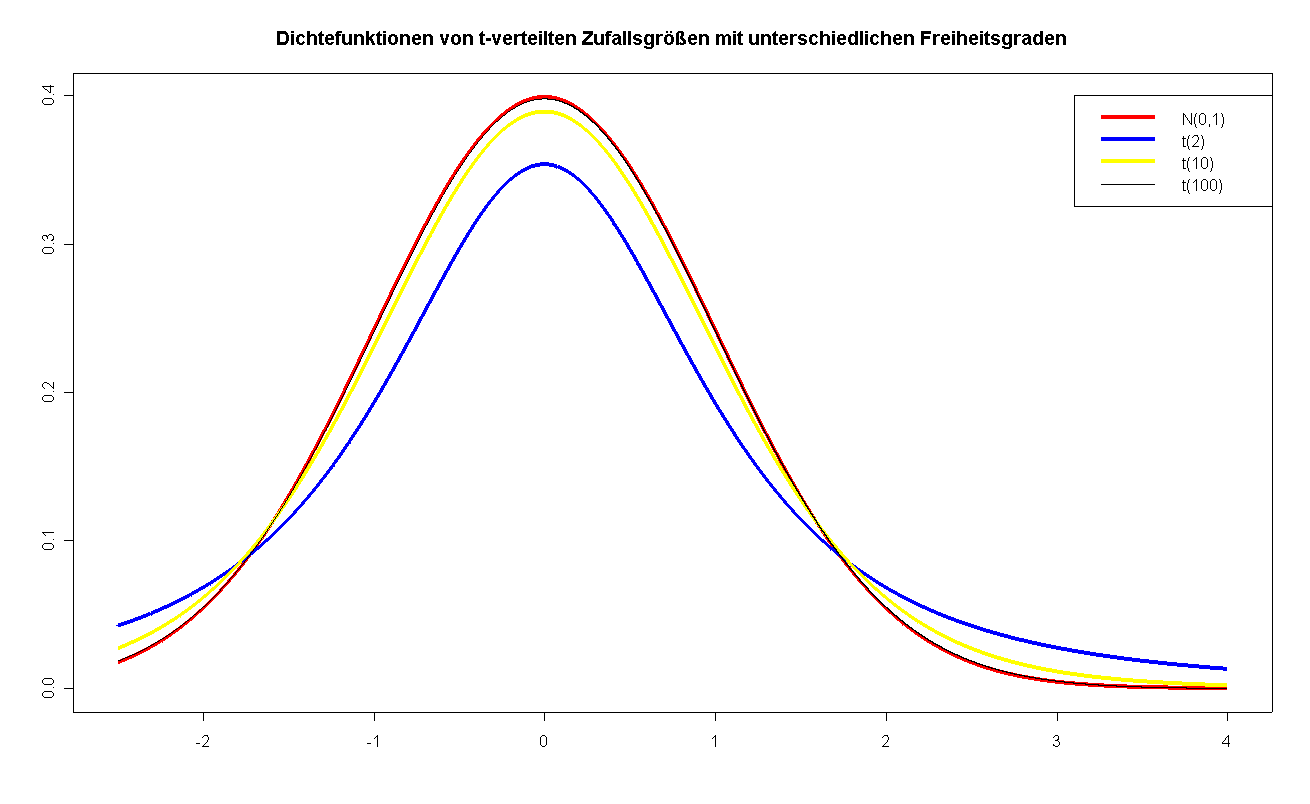
\includegraphics[width=8cm,height=4cm]{./bilder/T-Verteilung.png}\\
		$\lim\limits_{x\rightarrow \infty}$ = 0 aber langsamer wie bei
		Gaussverteilung 
    \end{minipage}

		\begin{tabular}{p{2cm}p{16cm}}
        Beispiel: & \textcolor{green}{10} Messungen ergeben Durchschnittswert
        \textcolor{red}{4{,}7} und eine Standardabweichung \textcolor{blue}{0{,}1}.
        Finde ein 99\%  Konfidenzintervall für $\mu$.\\
        
         Finde t: & \begin{tabular}{| c | c | c | c |}
                   \hline
                   $k=\textcolor{green}{n}-1$ & \ldots & 0{,}995\\
                   \hline
                   \vdots & \vdots & \vdots \\
                   \hline
                   9 & \ldots & 3{,}2498\\
                   \hline
                   \end{tabular}
        
       		 $\left[\textcolor{red}{\bar{X}}-3,2498\frac{\textcolor{blue}{S}}{\sqrt{\textcolor{green}{n}}},
		\textcolor{red}{\bar{X}}+3,2498\frac{\textcolor{blue}{S}}{\sqrt{\textcolor{green}{n}}}\right]
		\Rightarrow 
		\left[{\color{red}4{,}7}-3{,}2498\frac{\textcolor{blue}{0{,}1}}{\sqrt{\textcolor{green}{10}}},
		\textcolor{red}{4{,}7}+3{,}2498\frac{\textcolor{blue}{0{,}1}}{\sqrt{\textcolor{green}{10}}}\right]$\\ \\
		& $\mu\in \left[4{,}5072, 4{,}8028\right]$ mit Wahrscheinlichkeit 99\%
        \end{tabular}
\hrule

	\subsection{Konfidenzintervall \skript{139} \sachs{146}}
	\begin{tabular}{p{18cm}}
     Ein Intervall $[L(X_1,\ldots,X_n),R(X_1,\ldots,X_n)]$ heisst ein
     $1-\alpha$- Konfidenzintervall für den Parameter $\vartheta$, wenn der wahre
     Wert des Parameters $\vartheta$ höchstens mit Wahrscheinlichkeit $\alpha$
     ausserhalb des Intervalls liegt.
    \end{tabular}\\ 
 
\section{Hypothesentest \skript{143}}
	\subsection{Grundsätze}
	- ``Man braucht Aussagen, die man widerlegen könnte.''\\
	- Irrtum ist möglich (Irrtumsw'keit $\alpha$)\\
	- Beweis durch Widerlegen des Gegenbeweises
	\subsection{Vorgehen (Nullhypothese)}
	\begin{enumerate}
      \item Hypothese, die der Test \textbf{widerlegen} soll\\
      	$\rightarrow$ Nullhypothese $\Rightarrow$ Keine Wirkung/Effekt
      \item Festlegung der Irrtumswahrscheinlichkeit 	$\alpha$ = 0.05, 0.01, \ldots (Niveau=1-$\alpha$)
      \item Testgrösse X, W'keitsverteilung
      	$\rightarrow$ Nur Werte bis zum getesteten Ereignis betrachten! (Nicht Zukunft mit einbeziehen)
      \item Bestimmung der Schranken $x_{krit}$ für: 		
      	\begin{itemize}
      		\item Einseitiger Test $P(X > x_{krit})=\alpha$
      		\item Zweiseitiger Test $P(|X| > x_{krit})=\alpha/2$
      	\end{itemize}
      \item Wert für $F\!\left({\frac{x_{krit}-\mu}{\sigma}}\right)$ aus Tabelle 10.1
      %TODO pageref für Tabelle
      \item Falls Messungen ergeben $X > x_{krit} \Longrightarrow$ Hypothese
      \textbf{falsch} mit W'keit $1-\alpha$
    \end{enumerate}
    
    
	\subsection{Testen einer diskreten Verteilung
	\skript{147}}
	\subsubsection{$\chi^2$-Test mit k-möglichen Ausgängen}
		
		\begin{tabular}{l l}
			Mögliche Ausgänge: $I_i$, $i=1,\ldots,k$&
			Wahrscheinlichkeit von Ausgang $i$: $P(X\in I_i)=\textcolor{red}{p_i}$\\
			$n$ Beobachtungen, davon jeweils \textcolor{blue}{$n_i$} mit Ausgang $i$ &
			$\boxed{D=\sum\limits_{i=1}^{k}\frac{(\textcolor{blue}{n_i}-\textcolor{red}{np_i})^2}{\textcolor{red}{np_i}}}$ \hspace{4mm} ist $\chi^2_{k-1}$, mit $k-1$ Freiheitsgrade\\
		\end{tabular}
        
       % $\varphi_n(x)=  \begin{cases}\displaystyle \frac{x^{\frac{r}{2}-1}e^{
        %-\frac{x}{2}}}{2^{\frac{r}{2}}\Gamma\left(\frac{r}{2}\right)} & x>0 \\
        %0 & x\leq 0 \end{cases} $\\  
		%$E(X)=r; \quad var(X)=2r$

		
		\textbf{Durchführung des $\chi^2$-Tests}\\
		\begin{minipage}{13cm}
		\begin{tabular}{p{4cm}p{8cm}}
		1. Daten erfassen: &
			Damit der Test optimal funktioniert muss folgende Bedingung erfüllt sein:
			$\boldsymbol{n_i\geq 5 \; \forall \; i}$\\
        
        2. \textbf{Diskrepanz $D$} berechnen & \begin{tabular}[t]{|c|c|c|c|c|c|}
                                  \hline
                                  $i$ & Ausgang & $p_i$ & $n_i$ & $(n_i-np_i)$ &
                                  $(n_i-np_i)^2/np_i$\\
                                  \hline
                                  1 & & & & & \\
                                  2 & & & & & \\
                                  3 & & & & & \\
                                  4 & & & & & \\
                                  5 & & & & & \\
                                  \hline
                                  & & & n & & $D=\sum$ \\
                                  \hline
                                  
                                  \end{tabular}\\
        3. Schwellenwert für $D$ & $x_{1-\alpha}$ für $F_{\chi_{k-1}^2}(x) = 1- \alpha$ aus $\chi_{k-1}^2$-Tabelle lesen. \\
        & Wenn
        $\alpha$ nicht vorgegeben, dann $\alpha$ z.B. $0.1$ oder $0.05$
        wählen.\\
        &Anzahl Freiheitsgrade= Anzahl Ausgänge$ -1 $ = $k - 1$ \\ & $p=1-\alpha$ \hspace{10mm}$\alpha=$Irrtumswahrscheinlichkeit\\
        & \textcolor{green}{$D \geq x_{1-\alpha}$} Hypothese ist unwahrscheinlich!\\
        & $D < x_{1-\alpha}$ Hypothese nicht wiederlegbar!\\
        & \textcolor{blue}{$D \leq x_\alpha$} Daten möglicherweise
        ''fabriziert''!\\
        \end{tabular}
        \end{minipage}
		\begin{minipage}{6cm}
		\vspace*{6cm}
        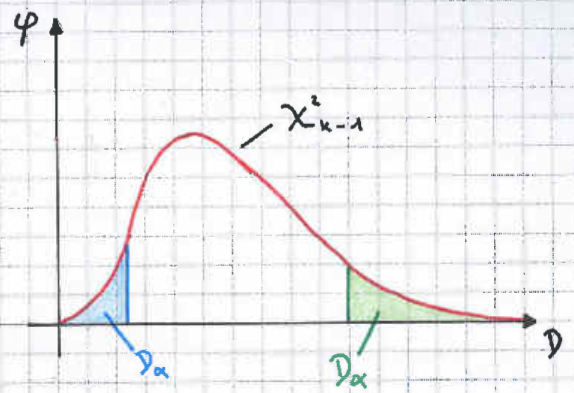
\includegraphics[width=6cm]{./bilder/chi-test.png}
        \end{minipage}\\
	\begin{tabular}{ll}
    	Nachteile:&	-Grob verpixeltes Bild der Verteilung\\
    	&			-wenn wenig Messwerte $\Longrightarrow$ geringe Aussagekraft
    \end{tabular}
   	
  \subsection{Testen einer stetigen Verteilung}
  	\subsubsection{Mit $\chi^2$-Test}
  	\begin{minipage}{13cm}
  		Der $\chi^2$-Test kann im Prinzip nur diskrete Wahrscheinlichkeitsverteilungen testen.\\
  		$\rightarrow$ Will man eine stetige Verteilung testen, muss man zunächst Klassen von Werten bilden. $\rightarrow$ Anschliessend deren Wahrscheinlichkeiten berechnen und dann prüfen ob die künstlich diskrete Verteilung im $\chi^2$-Test Bestand hat.\\
  		$\Rightarrow$ Achtung: Durch die Klassenbildung wird eine künstliche Diskretisierung eingeführt. 
  	\end{minipage}		
  	\begin{minipage}{6.5cm}
  	        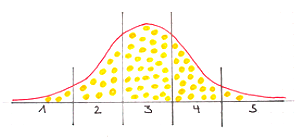
\includegraphics[width=6cm]{./bilder/chi_quadrat.png}\\
  	        \end{minipage}
  	        
  	
	\subsubsection{Kolmogorov-Smirnov Test}
	\begin{tabular}{ll}
	\textbf{Nullhypothese} & Messwerte $x_1, ..., x_n$ haben Verteilungsfunktion $F_X$\\
    Idee: & Vergleiche Verteilungsfunktionen (statt der Dichtefunktionen)\\
    Daten: & $X$ Zufallsvariable, Verteilungsfunktion $F_X$, $n$ Messungen
    ergeben Stichprobe $x_i$
    \end{tabular}

	\begin{minipage}{6cm}
    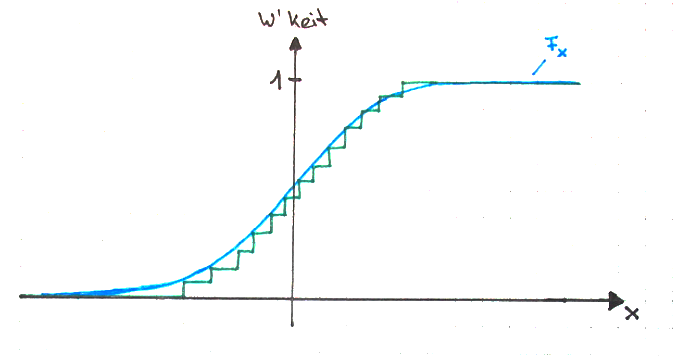
\includegraphics[width=6cm]{./bilder/ks1.png}\\
    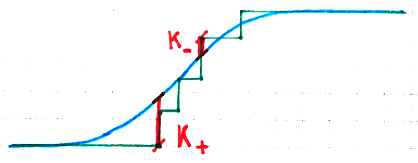
\includegraphics[width=6cm]{./bilder/ks2.png}\\
    \end{minipage}
	\begin{minipage}{12cm}
    \textcolor{blue}{$F_X$ theoretische Verteilungsfunktion von X}\\ \\
    \vspace{15mm}
    \textcolor{green}{empirische Verteilungsfunktion $\frac{Anzahl\{x_i \leq
    x \}}{n}$}\\

    Testgrösse\\
    \hspace*{0.5cm}
    	\parbox{6cm}{\textcolor{red}{max}
   			(\textcolor{green}{$F_{emp}$(x)} - 
   			\textcolor{blue}{$F_x$(x)})\\
    		\textcolor{red}{min} 
    		\textcolor{green}{$(F_{emp}(x)$}-
    		\textcolor{blue}{$F_x(x))$}}

    \end{minipage}

	\textbf{Durchführen des Kolmogorov-Smirnov Test}\\
	\begin{tabular}{l p{18cm}}
		1. &  Werte $x_1, ..., x_n$ in aufsteigender Reihenfolge sortieren\\
		2. & \parbox[t]{18cm}{
				$\mathbf{K_n^{\pm}}$ \textbf{berechnen}\\
				\hspace*{0.5cm}
				\parbox{6cm}{
					$\boxed{K_n^+ = \sqrt{n}\underset{1<x<n}{max}\left(\frac{i}{n} - F_X(x_i)\right)}$\\
					$\boxed{K_n^- = \sqrt{n}\underset{1<x<n}{max}\left(F_X(x_i)- \frac{i-1}{n}\right)}$}
				\parbox[c]{8cm}{
					Mit Tabelle:
					\begin{tabular}[t]{|c|c|c|c|c|}
				   		\hline
				    	$i$ & $x_i$ & $i/n$ & $F_X(x_i)$ & $(i-1)/n$ \\
				    	\hline
				    	1 & $min(x_i)$ & & & \\
				    	& $\vdots$ & & &\\	    
				    	n & $max(x_i)$ & & &\\
				     	\hline
				     
				 \end{tabular}
				 }		
		}\\
	3. & Finde $t_{n,1-\alpha}$,$t_{n,\alpha}$  in der Tabelle 10.3\\
	%TODO Pageref für Tabelle
	4. & Falls $K^+_n > t_{n,1-\alpha}$ oder $K^-_n < t_{n,\alpha}$,
			verwerfe die Hypothese, dass $X$ die Verteilungsfunktion $F_X$ hat. 
	\end{tabular}

\subsection{Vergleichen von Mittelwerten (t-Test)}
	\begin{tabular}{l l}
		\textbf{Nullhypothese} & 
		$\Rightarrow$ $E(X) = E(Y)$\\
		
		\textbf{Daten}&
		$\mathbf{n}$ Messungen von $x_i \Rightarrow \bar{X} \; ; \; S_X^2$ \\ 
		& $\mathbf{m}$ Messungen von $y_i \Rightarrow \bar{Y} \; ; \; S_Y^2$\\
		
		\textbf{Testgrösse} &
		$T = \dfrac{\bar{X}-\bar{Y}}{\sqrt{(n-1)\cdot S_X^2 + (m-1)\cdot S_Y^2}}\cdot \sqrt{\dfrac{n m (n+m-2)}{n + m}}$\\
		& T ist t-verteilt\\
		
		\textbf{Schwellenwert} &
		$t_{krit}$ aus Tabelle 10.4 mit Freiheitsgrad $n+m-2$ und $p = 1-\alpha$\\
		%TODO Pageref für Tabelle
		
		\textbf{Test} &
		Falls $T > t_{krit}$ wird die Hypothese $E(X) = E(Y)$ verworfen
		
	\end{tabular}
	 
	
	
	\

\input{sections/Kalman}

\section{Wichtige Formeln}
\input{idiotenseite/diverses/subsections/Reihenentwicklung}
\newpage
\section{Auswahl der Verteilung}

	\begin{tabular}{|l|p{12cm}|}
	\hline
		Gleichverteilung &
			Alle möglichen Werte haben die gleiche Wahrscheinlichkeit \\
	\hline	
		Exponentialverteilung &
			Dauer von zufälligen Zeitintervallen ohne Gedächtnis \\
	\hline
		Normalverteilung &
			Viele kleine, unabhängige Zufallsprozesse sammeln sich zu einer normalverteilten Zufallsvariable \\
	\hline			
		Binomialverteilung &
			Experiment mit zwei Ausgängen \\
	\hline			
		Hypergeometrische Verteilung &
			Wahrscheinlichkeit, dass in einer Stichprobe, Elemente einer Teilmenge zu finden sind \\
	\hline	
		Poissonverteilung &
			Häufigkeiten seltener Ereignisse \\
	\hline
		t-Verteilung &
			Varianz aus Stichproben geschätzt (für grosse $n$ kann Normalverteilung verwendet werden)\\
	\hline
		$\chi^2$-Verteilung &
			Test ob eine Zufallsvariable Normalverteilt ist. Anwendung bei Hypothesentests\\
	\hline
	\end{tabular}
\section{Übungsverzeichnis}
\begin{center}
\begin{tabular}{|l|l|l|}
\hline
\textbf{Titel} & \textbf{Beschreibung} & \textbf{Übungsnummer} \\ \hline
$\chi^2$-Test & M\&M's Experiment & 12.1 \\ \hline
4 Damen und 5 Her. auf 9 Stühle Platz. & Verschiedene Ereignisse die Auftreten auflisten & 3.1 \\ \hline
Alzheimer-Test & Bedingte W'keit, Satz der totalen W'keit & 2.4 \\ \hline
Auto-Ziegen-Problem & Monty-Hall Problem & 4.1, 4.2, 4.3 \\ & & 5.1 (mit Gewinn) \\ \hline
Beweis Poisson-Verteilung & Bewieiss, dass PV wirklich eine W'keitsverteilung ist & 10.2 \\ \hline
Buch mit n Seiten und f Druckfehlern & Poisson-Verteilung, W'keit genau 2 Fehler auf einer Seite & 10.1 \\ \hline
Dichtefunktion mit unb. Parameter & Parameter, $F(x)$, $E(x)$, $Var(x)$ und Abw. von $E(x)$ berech. & 7.3, 10.4 \\ \hline
Epidemie auf Kleinplanet Zürch & ein paar der infiz. Bewohner werden untersucht & 3.5 \\ \hline
EW einer sym. Dichtefunktion & & 7.2 \\ \hline
Exp.verteilte ZV mit unb. Parameter & $Var(x)$ berechnen & 8.1 \\ \hline
Faire Münze mehrmals werfen & W'keiten der möglichen Werte und $E(x)$ berechnen & 5.3 \\ \hline 
Faire Münze mit Gewinn & Gewinn entspricht der (k+1)-ten Primzahl & 5.2 \\ \hline
Fairer Würfel n mal geworfen & W'keit mehr als 15 von 100 6er abzuweichen & 10.5 \\ \hline
Familie mit Kindern & Versch. Ereignisse die Auftreten auflisten & 2.2 \\ \hline
Funktionsf. eines Gerätes (krit. Bauteil) & Ausfall des Bauteils inn. der ersten Woche & 8.3 \\ \hline
Game-Controller & Schätzwert für Drehgeschwindigkeit & 13.2 \\ \hline
Gleichverteilte Zufallsvariable & Erwartungswert und Verteilungsfunktion berechnen & 7.4 \\ \hline
Gleichverteilte ZV & Intervall [0,1], $F(x)$, $\varphi(x)$, $E(x) $ und $var(x)$ & 8.2 \\ \hline
Glücksrad & Spielfolgen & 2.1 \\ \hline
Google-Matrix & Besuchsw'keiten anhand von Link-Struktur bestimmen & 4.5 \\ \hline
Hüte und Lose & 2 Hüte mit untersch. Lose und Nieten & 3.4 \\ \hline
Hypergeometrische Verteilung & Prozess wegen Diskriminierung & 12.3 \\ \hline
Hypotese Testen & Zahlen sollen angeblich Exponentialv. sein mit Parameter & 13.1 \\ \hline
Impfexperiment & W'keit, dass Individuum Komplik. hat, Poisson-Verteilung & 10.3 \\ \hline
Kalman-Filter & Konstruktion & 13.3, 13.4 \\ \hline
Kursteilnehmer in 4er-Gruppen eint. & vieviele versch. Arten gibt es & 3.3 \\ \hline
Laborversuch, geg. $Var(x)$ & Resultat soll bis zu einer Stelle nach dem Komma genau sein & 7.1 \\ \hline
M\&M's Experiment & $\chi^2$  Wird eine Fabe bevorzugt?  & 12.1 \\ \hline
Maschinene die Bauteile produziert & Maschinen produzieren untschersch. Ausschuss & 4.4 \\ \hline
Mengen & Visualisieren von Ereignissen & 1.1, 1.2 \\ \hline
Monty-Hall Problem & Auto-Ziegen-Problem & 4.1, 4.2, 4.3 \\ & & 5.1 (mit Gewinn) \\ \hline
Multiple Choice Test & 10 Fragen a je 3 Antworten & 3.5 \\ \hline
Numbers mit Morde in Grossstadt & & 11.1 \\ \hline
Prozess wegen Diskriminierung & hypergeometrische Verteilung & 12.3 \\ \hline
Raketenexperiment Müller & Meth. der kleins. Quad. um approx. der Datenp. zu kriegen & 9.6 \\ \hline
Schätzer finden & & 11.2 - 11.4 \\ \hline
Schätzer mit Param. der Exp.vert. & Schätzer entw. konsistend und/oder erwartungstreu & 11.2 \\ \hline
Sensor-, Server-Problem & Lineare Regression durchführen neue Werte zu finden & 6.6 \\ \hline
Sitzordnungen & vieviele Sitzordnungen bei n-Personen möglich sind & 3.2 \\ \hline
Sorte Körnermais liefert Ertrag & empirische Standardabweichung, 95\%-Quantile der Normalv. & 9.2 \\ \hline
Standardnormalvert. ZV& $P(-0.46 \leq X \leq 0.21)$ berechnen & 9.1 \\ \hline
Streng mon. Wachsende $F(x)$ & $F(x)$ einer anderen Zufallsvariablen berechenen & 7.5 \\ \hline
Unfaire Münze & n Würfe und daraus Erwartungswert und Varianz berechnen & 6.3 \\ \hline
Unfairer Würfel & Erwartungswert und Varianz der Augenzahl berechnene & 6.1 \\ \hline
Wahrscheinlichkeitsmaschine & generiert ganze Zufallszahlen >= 0 & 5.4 \\ \hline
Webseite mit Besucherzahlen & Hypothese und Normalverteilung & 12.2 \\ \hline
Wendep. der Normalv. bestimmem & $P(x_{-} \leq X \leq x_{+})$  berechnen & 9.5
\\ \hline Würfel wird n-mal geworfen & W'keit, dass bei $n=100$ die Augens. zwischen $320-360$ & 9.4 \\ \hline
Zementsäcke à $1$kg mit Standardabw. & W'keit dass Sack weniger wie 99.4 kg Inhalt hat & 9.3 \\ \hline
Zufallsvariable mit Werten 0 oder 1 & Erwartungswert und Varianz berechnen & 6.2 \\ \hline
\end{tabular}
\end{center}
\newpage
\renewcommand{\arraystretch}{1}
\section{Tabellen}
\copyright$\;$ Prof. Dr. Andreas Müller
\subsection{Quantilen der Normalverteilung}
	\begin{minipage}{18cm}
    	\centering
    	\scriptsize
\begin{tabular}{|l|r|}
\hline
$p$&$x$\\
\hline
0.75&0.6745\\
0.8&0.8416\\
0.9&1.2816\\
0.95&1.6449\\
0.975&1.9600\\
0.99&2.3263\\
0.995&2.5758\\
0.999&3.0902\\
0.9995&3.2905\\
\hline
\end{tabular}
    \end{minipage}

	\subsection{Verteilungsfunktion der Normalverteilung}
	\begin{minipage}{18cm}
    	\centering
        \scriptsize
\begin{tabular}{|r|rrrrrrrrrr|}
\hline
$x$&+0.00&+0.01&+0.02&+0.03&+0.04&+0.05&+0.06&+0.07&+0.08&+0.09\\
\hline
0.0&0.5000&0.5040&0.5080&0.5120&0.5160&0.5199&0.5239&0.5279&0.5319&0.5359\\
0.1&0.5398&0.5438&0.5478&0.5517&0.5557&0.5596&0.5636&0.5675&0.5714&0.5753\\
0.2&0.5793&0.5832&0.5871&0.5910&0.5948&0.5987&0.6026&0.6064&0.6103&0.6141\\
0.3&0.6179&0.6217&0.6255&0.6293&0.6331&0.6368&0.6406&0.6443&0.6480&0.6517\\
0.4&0.6554&0.6591&0.6628&0.6664&0.6700&0.6736&0.6772&0.6808&0.6844&0.6879\\
0.5&0.6915&0.6950&0.6985&0.7019&0.7054&0.7088&0.7123&0.7157&0.7190&0.7224\\
0.6&0.7257&0.7291&0.7324&0.7357&0.7389&0.7422&0.7454&0.7486&0.7517&0.7549\\
0.7&0.7580&0.7611&0.7642&0.7673&0.7704&0.7734&0.7764&0.7794&0.7823&0.7852\\
0.8&0.7881&0.7910&0.7939&0.7967&0.7995&0.8023&0.8051&0.8078&0.8106&0.8133\\
0.9&0.8159&0.8186&0.8212&0.8238&0.8264&0.8289&0.8315&0.8340&0.8365&0.8389\\
1.0&0.8413&0.8438&0.8461&0.8485&0.8508&0.8531&0.8554&0.8577&0.8599&0.8621\\
1.1&0.8643&0.8665&0.8686&0.8708&0.8729&0.8749&0.8770&0.8790&0.8810&0.8830\\
1.2&0.8849&0.8869&0.8888&0.8907&0.8925&0.8944&0.8962&0.8980&0.8997&0.9015\\
1.3&0.9032&0.9049&0.9066&0.9082&0.9099&0.9115&0.9131&0.9147&0.9162&0.9177\\
1.4&0.9192&0.9207&0.9222&0.9236&0.9251&0.9265&0.9279&0.9292&0.9306&0.9319\\
1.5&0.9332&0.9345&0.9357&0.9370&0.9382&0.9394&0.9406&0.9418&0.9429&0.9441\\
1.6&0.9452&0.9463&0.9474&0.9484&0.9495&0.9505&0.9515&0.9525&0.9535&0.9545\\
1.7&0.9554&0.9564&0.9573&0.9582&0.9591&0.9599&0.9608&0.9616&0.9625&0.9633\\
1.8&0.9641&0.9649&0.9656&0.9664&0.9671&0.9678&0.9686&0.9693&0.9699&0.9706\\
1.9&0.9713&0.9719&0.9726&0.9732&0.9738&0.9744&0.9750&0.9756&0.9761&0.9767\\
2.0&0.9772&0.9778&0.9783&0.9788&0.9793&0.9798&0.9803&0.9808&0.9812&0.9817\\
2.1&0.9821&0.9826&0.9830&0.9834&0.9838&0.9842&0.9846&0.9850&0.9854&0.9857\\
2.2&0.9861&0.9864&0.9868&0.9871&0.9875&0.9878&0.9881&0.9884&0.9887&0.9890\\
2.3&0.9893&0.9896&0.9898&0.9901&0.9904&0.9906&0.9909&0.9911&0.9913&0.9916\\
2.4&0.9918&0.9920&0.9922&0.9925&0.9927&0.9929&0.9931&0.9932&0.9934&0.9936\\
2.5&0.9938&0.9940&0.9941&0.9943&0.9945&0.9946&0.9948&0.9949&0.9951&0.9952\\
2.6&0.9953&0.9955&0.9956&0.9957&0.9959&0.9960&0.9961&0.9962&0.9963&0.9964\\
2.7&0.9965&0.9966&0.9967&0.9968&0.9969&0.9970&0.9971&0.9972&0.9973&0.9974\\
2.8&0.9974&0.9975&0.9976&0.9977&0.9977&0.9978&0.9979&0.9979&0.9980&0.9981\\
2.9&0.9981&0.9982&0.9982&0.9983&0.9984&0.9984&0.9985&0.9985&0.9986&0.9986\\
3.0&0.9987&0.9987&0.9987&0.9988&0.9988&0.9989&0.9989&0.9989&0.9990&0.9990\\
\hline
\end{tabular}
    \end{minipage}

	\subsection{Quantilen für den Kolmogorov-Smirnov-Test}
	\begin{minipage}{18cm}
    	\centering
    	\scriptsize
\begin{tabular}{|r|rrr|rrr|rrr|}
\hline
$n$&$p=0.01$&$p=0.05$&$p=0.1$&$p=0.25$&$p=0.5$&$p=0.75$&$p=0.9$&$p=0.95$&$p=0.99$\\
\hline
1&0.01000&0.05000&0.10000&0.25000&0.50000&0.75000&0.90000&0.95000&0.99000\\
2&0.01400&0.06749&0.12955&0.29289&0.51764&0.70711&0.96700&1.09799&1.27279\\
3&0.01699&0.07919&0.14714&0.31117&0.51469&0.75394&0.97828&1.10166&1.35889\\
4&0.01943&0.08789&0.15899&0.32023&0.51104&0.76419&0.98531&1.13043&1.37774\\
5&0.02152&0.09471&0.16750&0.32490&0.52449&0.76741&0.99948&1.13916&1.40242\\
6&0.02336&0.10022&0.17385&0.32717&0.53193&0.77028&1.00520&1.14634&1.41435\\
7&0.02501&0.10479&0.17873&0.32804&0.53635&0.77552&1.00929&1.15373&1.42457\\
8&0.02650&0.10863&0.18256&0.32802&0.53916&0.77971&1.01346&1.15859&1.43272\\
9&0.02786&0.11191&0.18560&0.32745&0.54109&0.78246&1.01731&1.16239&1.43878\\
10&0.02912&0.11473&0.18803&0.32975&0.54258&0.78454&1.02016&1.16582&1.44397\\
11&0.03028&0.11718&0.19000&0.33304&0.54390&0.78633&1.02249&1.16885&1.44837\\
12&0.03137&0.11933&0.19160&0.33570&0.54527&0.78802&1.02458&1.17139&1.45207\\
13&0.03239&0.12123&0.19291&0.33789&0.54682&0.78966&1.02649&1.17357&1.45527\\
14&0.03334&0.12290&0.19396&0.33970&0.54856&0.79122&1.02823&1.17552&1.45810\\
15&0.03424&0.12439&0.19482&0.34122&0.55002&0.79259&1.02977&1.17728&1.46060\\
16&0.03509&0.12573&0.19552&0.34250&0.55123&0.79377&1.03113&1.17888&1.46283\\
17&0.03589&0.12692&0.19607&0.34360&0.55228&0.79482&1.03237&1.18032&1.46483\\
18&0.03665&0.12799&0.19650&0.34454&0.55319&0.79578&1.03351&1.18162&1.46664\\
19&0.03738&0.12895&0.19684&0.34535&0.55400&0.79667&1.03457&1.18282&1.46830\\
20&0.03807&0.12982&0.19709&0.34607&0.55475&0.79752&1.03555&1.18392&1.46981\\
30&0.04354&0.13510&0.20063&0.35087&0.56047&0.80362&1.04243&1.19164&1.48009\\
50&0.05005&0.13755&0.20794&0.35713&0.56644&0.80988&1.04933&1.19921&1.48969\\
100&0.05698&0.14472&0.21370&0.36331&0.57269&0.81634&1.05627&1.20666&1.49864\\
200&0.06049&0.14887&0.21816&0.36784&0.57725&0.82099&1.06117&1.21180&1.50458\\

\hline
\end{tabular}

    \end{minipage}
\newpage

	\subsection{Quantilen der t-Verteilung}
	\begin{minipage}{18cm}
    	\centering
    	\scriptsize
 \begin{tabular}{|r|rrrrrrr|}
\hline
$k = n-1$&0.75&0.8&0.9&0.95&0.975&0.99&0.995\\
\hline
1&1.0000&1.3764&3.0777&6.3138&12.7062&31.8205&63.6567\\
2&0.8165&1.0607&1.8856&2.9200&4.3027&6.9646&9.9248\\
3&0.7649&0.9785&1.6377&2.3534&3.1824&4.5407&5.8409\\
4&0.7407&0.9410&1.5332&2.1318&2.7764&3.7469&4.6041\\
5&0.7267&0.9195&1.4759&2.0150&2.5706&3.3649&4.0321\\
6&0.7176&0.9057&1.4398&1.9432&2.4469&3.1427&3.7074\\
7&0.7111&0.8960&1.4149&1.8946&2.3646&2.9980&3.4995\\
8&0.7064&0.8889&1.3968&1.8595&2.3060&2.8965&3.3554\\
9&0.7027&0.8834&1.3830&1.8331&2.2622&2.8214&3.2498\\
10&0.6998&0.8791&1.3722&1.8125&2.2281&2.7638&3.1693\\
11&0.6974&0.8755&1.3634&1.7959&2.2010&2.7181&3.1058\\
12&0.6955&0.8726&1.3562&1.7823&2.1788&2.6810&3.0545\\
13&0.6938&0.8702&1.3502&1.7709&2.1604&2.6503&3.0123\\
14&0.6924&0.8681&1.3450&1.7613&2.1448&2.6245&2.9768\\
15&0.6912&0.8662&1.3406&1.7531&2.1314&2.6025&2.9467\\
16&0.6901&0.8647&1.3368&1.7459&2.1199&2.5835&2.9208\\
17&0.6892&0.8633&1.3334&1.7396&2.1098&2.5669&2.8982\\
18&0.6884&0.8620&1.3304&1.7341&2.1009&2.5524&2.8784\\
19&0.6876&0.8610&1.3277&1.7291&2.0930&2.5395&2.8609\\
20&0.6870&0.8600&1.3253&1.7247&2.0860&2.5280&2.8453\\
21&0.6864&0.8591&1.3232&1.7207&2.0796&2.5176&2.8314\\
22&0.6858&0.8583&1.3212&1.7171&2.0739&2.5083&2.8188\\
23&0.6853&0.8575&1.3195&1.7139&2.0687&2.4999&2.8073\\
24&0.6848&0.8569&1.3178&1.7109&2.0639&2.4922&2.7969\\
25&0.6844&0.8562&1.3163&1.7081&2.0595&2.4851&2.7874\\
26&0.6840&0.8557&1.3150&1.7056&2.0555&2.4786&2.7787\\
27&0.6837&0.8551&1.3137&1.7033&2.0518&2.4727&2.7707\\
28&0.6834&0.8546&1.3125&1.7011&2.0484&2.4671&2.7633\\
29&0.6830&0.8542&1.3114&1.6991&2.0452&2.4620&2.7564\\
30&0.6828&0.8538&1.3104&1.6973&2.0423&2.4573&2.7500\\
50&0.6794&0.8489&1.2987&1.6759&2.0086&2.4033&2.6778\\
100&0.6770&0.8452&1.2901&1.6602&1.9840&2.3642&2.6259\\
500&0.6750&0.8423&1.2832&1.6479&1.9647&2.3338&2.5857\\
$10^3$&0.6747&0.8420&1.2824&1.6464&1.9623&2.3301&2.5808\\
$10^4$&0.6745&0.8417&1.2816&1.6450&1.9602&2.3267&2.5763\\
$10^5$&0.6745&0.8416&1.2816&1.6449&1.9600&2.3264&2.5759\\
$10^6$&0.6745&0.8416&1.2816&1.6449&1.9600&2.3264&2.5758\\
\hline
\end{tabular}
    \end{minipage}


	\subsection{Quantilen der $\chi^2$-Verteilung}
	\begin{minipage}{18cm}
    \scriptsize
\begin{center}
\begin{tabular}{|r|rrr|rrr|rrr|}
\hline
\strut$k = n-1$&$p=0.01$&$p=0.05$&$p=0.1$&$p=0.25$&$p=0.5$&$p=0.75$&$p=0.9$&$p=0.95$&$p=0.99$\\
\hline
1&0.000&0.004&0.016&0.102&0.455&1.323&2.706&3.841&6.635\\
2&0.020&0.103&0.211&0.575&1.386&2.773&4.605&5.991&9.210\\
3&0.115&0.352&0.584&1.213&2.366&4.108&6.251&7.815&11.345\\
4&0.297&0.711&1.064&1.923&3.357&5.385&7.779&9.488&13.277\\
5&0.554&1.145&1.610&2.675&4.351&6.626&9.236&11.070&15.086\\
6&0.872&1.635&2.204&3.455&5.348&7.841&10.645&12.592&16.812\\
7&1.239&2.167&2.833&4.255&6.346&9.037&12.017&14.067&18.475\\
8&1.646&2.733&3.490&5.071&7.344&10.219&13.362&15.507&20.090\\
9&2.088&3.325&4.168&5.899&8.343&11.389&14.684&16.919&21.666\\
10&2.558&3.940&4.865&6.737&9.342&12.549&15.987&18.307&23.209\\
11&3.053&4.575&5.578&7.584&10.341&13.701&17.275&19.675&24.725\\
12&3.571&5.226&6.304&8.438&11.340&14.845&18.549&21.026&26.217\\
13&4.107&5.892&7.042&9.299&12.340&15.984&19.812&22.362&27.688\\
14&4.660&6.571&7.790&10.165&13.339&17.117&21.064&23.685&29.141\\
15&5.229&7.261&8.547&11.037&14.339&18.245&22.307&24.996&30.578\\
16&5.812&7.962&9.312&11.912&15.338&19.369&23.542&26.296&32.000\\
17&6.408&8.672&10.085&12.792&16.338&20.489&24.769&27.587&33.409\\
18&7.015&9.390&10.865&13.675&17.338&21.605&25.989&28.869&34.805\\
19&7.633&10.117&11.651&14.562&18.338&22.718&27.204&30.144&36.191\\
20&8.260&10.851&12.443&15.452&19.337&23.828&28.412&31.410&37.566\\
21&8.897&11.591&13.240&16.344&20.337&24.935&29.615&32.671&38.932\\
22&9.542&12.338&14.041&17.240&21.337&26.039&30.813&33.924&40.289\\
23&10.196&13.091&14.848&18.137&22.337&27.141&32.007&35.172&41.638\\
24&10.856&13.848&15.659&19.037&23.337&28.241&33.196&36.415&42.980\\
25&11.524&14.611&16.473&19.939&24.337&29.339&34.382&37.652&44.314\\
26&12.198&15.379&17.292&20.843&25.336&30.435&35.563&38.885&45.642\\
27&12.879&16.151&18.114&21.749&26.336&31.528&36.741&40.113&46.963\\
28&13.565&16.928&18.939&22.657&27.336&32.620&37.916&41.337&48.278\\
29&14.256&17.708&19.768&23.567&28.336&33.711&39.087&42.557&49.588\\
30&14.953&18.493&20.599&24.478&29.336&34.800&40.256&43.773&50.892\\
50&29.707&34.764&37.689&42.942&49.335&56.334&63.167&67.505&76.154\\
100&70.065&77.929&82.358&90.133&99.334&109.141&118.498&124.342&135.807\\
500&429.388&449.147&459.926&478.323&499.333&520.950&540.930&553.127&576.493\\
1000&898.912&927.594&943.133&969.484&999.333&1029.790&1057.724&1074.679&1106.969\\
\hline
\end{tabular}
\end{center}
    \end{minipage}
\renewcommand{\arraystretch}{\arraystretchOriginal}

%\section{Statistik mit dem Taschenrechner}
% Anderes Symbol für zuweisung: $\blacktriangleright$

\begin{center}
\begin{tabular}{|p{4cm}|p{11cm}|} \hline
\textbf{Funktion/Aufgabe} & \textbf{Eingabe} \\ \hline
$\binom{n}{k}$ & \tt{nCr(n,k)} \\ \hline
$\binom{n}{k}\cdot k!$ & \tt{nPr(n,k)} \\ \hline
Mittelwert $\overline{X}$ (konsistenter Schätzer) &
\tt{mean(\{}$x_1,\ldots,x_n$\tt{\})} \\ \hline
Standardabweichung $\sigma$ & \tt{stdDev($\{x_1, \ldots, x_n\}$)} \\ \hline
Varianz $\sigma^2$ & \tt{variance($\{x_1, \ldots, x_n\}$)} \\ \hline
Statistik anzeigen (berechnet folgende Werte: $ \bar x, \: \sum x, \: \sum x^2, \: \sigma x, \: ...$ &
\begin{minipage}[c]{11cm}\texttt{$\{x_1, \ldots, x_n\} \rightarrow$ l1} \\
					  \texttt{OneVar l1} \end{minipage} \\ \hline

Lineare Regression &     
\begin{list}{$\bullet$}{\setlength{\itemsep}{0cm}
	\setlength{\parsep}{0cm} \setlength{\topsep}{0cm}}  
	\item Vorbereitung:\newline
		\texttt{
			$\{x_1, \ldots, x_n\} \rightarrow$ l1;
			$\{y_1, \ldots, y_n\} \rightarrow$ l2;
			LinReg l1,l2}
	 \item Anzeige von Werten mit \newline \texttt{ShowStat}
	 \item Anzeige des Graphs mit \newline
	 	\texttt{regeq(x)}$\rightarrow$\texttt{y1(x)}$; \;$
	    \texttt{NewPlot 1,1,l1,l2}
\end{list} \\ \hline


\end{tabular}
\end{center}
\input{TI-Reference/tex/statistik}

\end{document} 
